\documentclass{beamer}
\usepackage[utf8]{inputenc}
\usepackage{appendixnumberbeamer}
\usepackage{graphicx}
\usepackage{ragged2e}
\usepackage{subcaption}

\usetheme[progressbar=frametitle]{metropolis}

% Prima pagina
\title{Malware analysis ``sample2.exe''}
\subtitle{}
\date{9 Gennaio 2020}
\author{Filippo Contro \hspace{3.8mm}{\scriptsize VR437055}\\ {\small\hspace{2.5mm} Michele Martini \hspace{2mm}{\scriptsize VR437056}}\vspace{1em}}


\begin{document}
\maketitle

\justify % Giustifica il testo a seguire

\begin{frame}{Summary}
	Simple calculator app

	\begin{figure}[h]
		\centering
		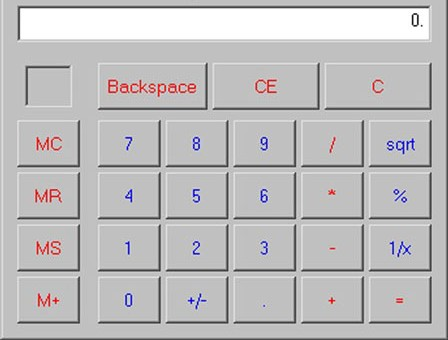
\includegraphics[height=12em]{../img/calculator.jpg}
	\end{figure}
	
	But under the hood\dots
\end{frame}

\begin{frame}
	\frametitle{Summary}
	\begin{itemize}
		\item Post requests
		\item Security center deactivation
		\item Infection \pause $\longrightarrow$ Polymorphic malware
	\end{itemize}
\end{frame}

%===============================================================================
\section{Static analysis}
\begin{frame}{Static analysis}
	First look

	\begin{figure}[h]
		\centering
		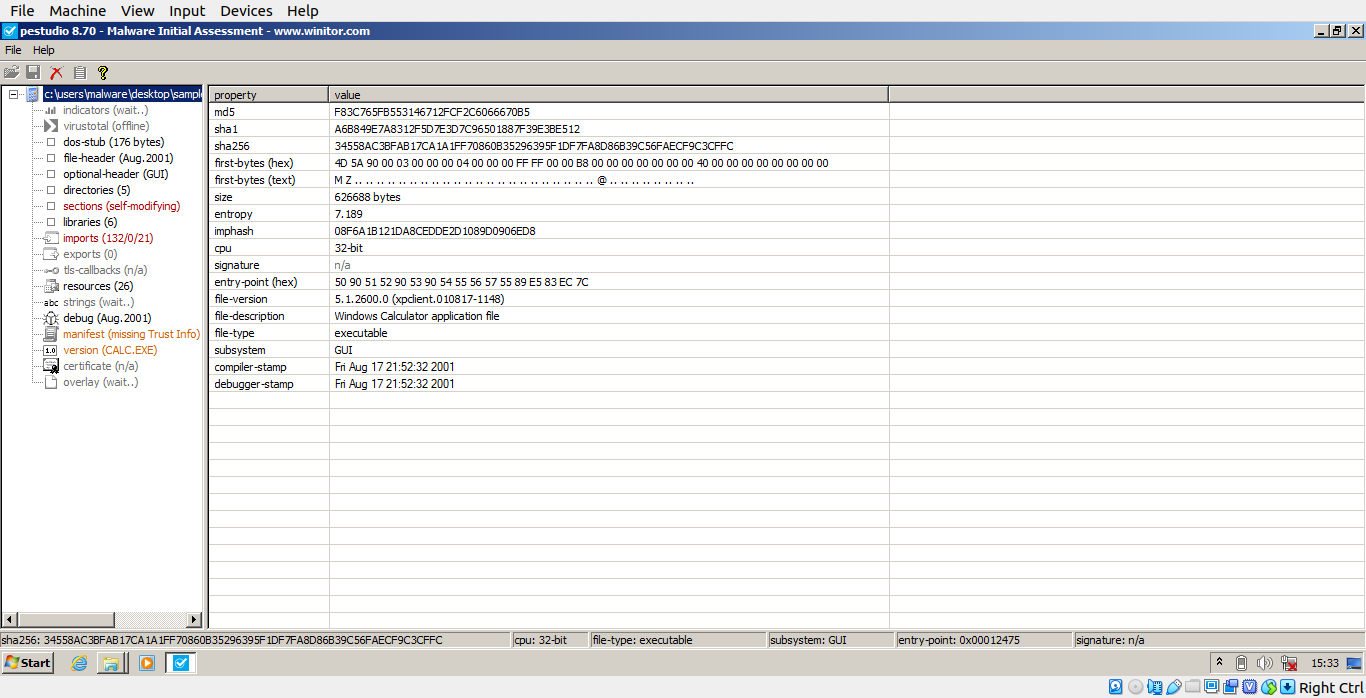
\includegraphics[height=12em]{../img/PEStudio-main.png}
	\end{figure}

	\pause

	High entropy \pause $\longrightarrow$ Obfuscation or Packing?
	
	\pause

	Let's look at the sections
\end{frame}
%-------------------------------------------------------------------------------

\begin{frame}{Sections}
	
	\begin{figure}[h]
		\centering
		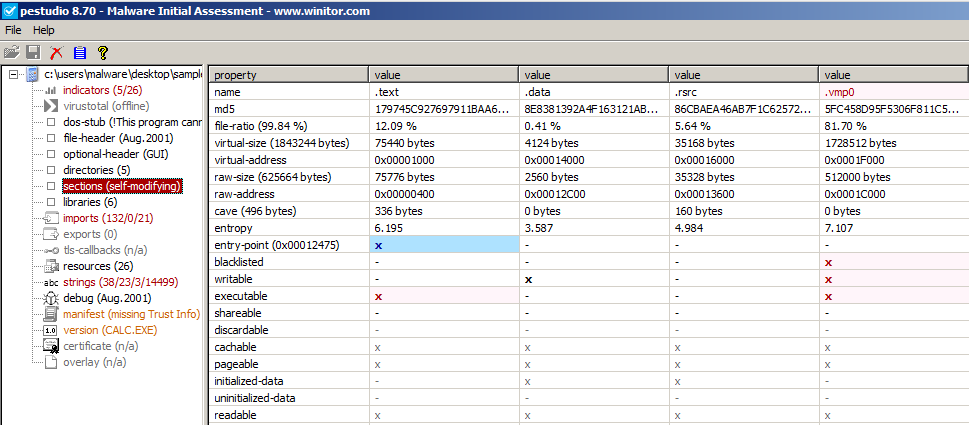
\includegraphics[height=12em]{../img/PEStudio-sections.png}
	\end{figure}

	The first three sections are OK!
	But \textbf{.vmp0} NO!
\end{frame}
%-------------------------------------------------------------------------------

\begin{frame}{Sections}
	\begin{figure}[h]
		\centering
		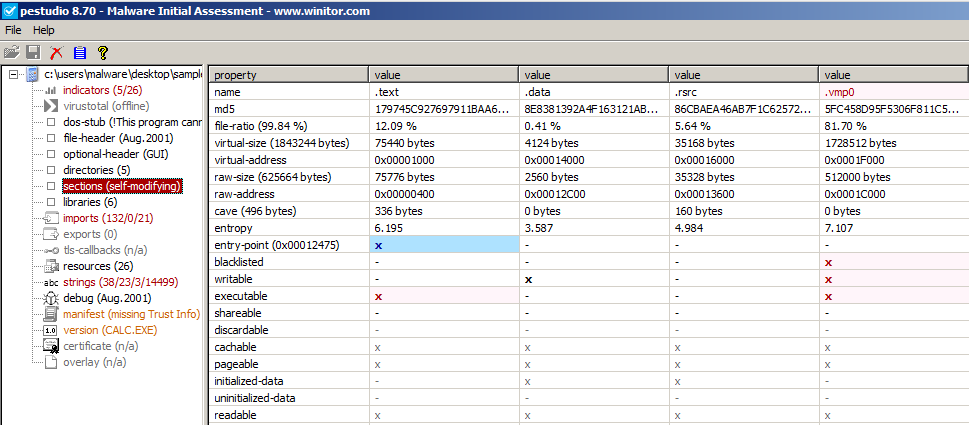
\includegraphics[height=12em]{../img/PEStudio-sections.png}
	\end{figure}
	\begin{itemize}
		\item High entropy
		\item Big portion of code (87\%)
		\item Both writable and executable \pause $\longrightarrow$ Very suspicious
	\end{itemize}
\end{frame}
%-------------------------------------------------------------------------------

\begin{frame}{Obfuscation}
	The presence of the 3 main sections (text, data, resources) suggests the absence of packing.
	
	\pause

	\begin{figure}[h]
		\centering
		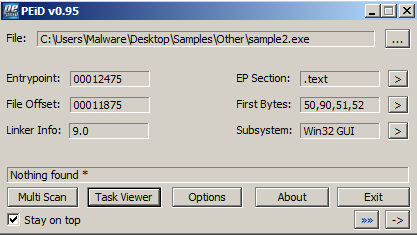
\includegraphics[height=12em]{../img/PEiD.png}
	\end{figure}
	PeID confirms our supposition.
	\pause
	
	The name \textbf{vmp0} is given by \textbf{VMProtect}.
\end{frame}
%-------------------------------------------------------------------------------

\begin{frame}{Imports}
	\begin{figure}[h]
		\centering
		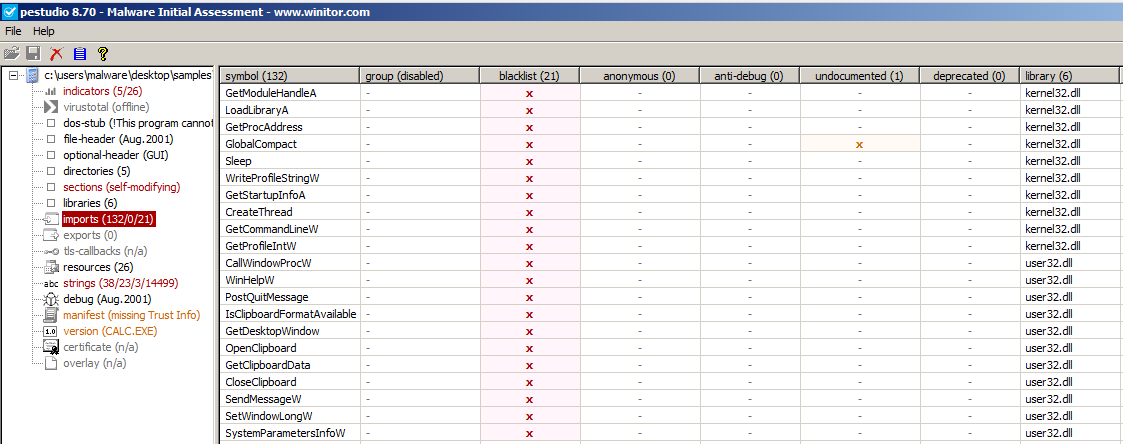
\includegraphics[height=8em]{../img/PEStudio-imports.png}
	\end{figure}

	The most interesting are

	\begin{itemize}
		\item getModuleHandleA
		\item loadLibraryA
		\item getProcAddressA
		\item getStartupInfoA
		\item getCommandLineW
	\end{itemize}
	\pause
	Other dealing with \textbf{Threads}, \textbf{Clipboard}, \textbf{System}
\end{frame}
%-------------------------------------------------------------------------------

\begin{frame}{Other}
	\begin{itemize}
		\item \textbf{Version}: Legit information, but no date
		\item \textbf{Strings}: Thousands of crypted strings
		\item \textbf{Certificate}: it is missing 
	\end{itemize}
\end{frame}

%-------------------------------------------------------------------------------

%===============================================================================
\section{Dynamic analysis}
\begin{frame}{Dynamic analysis}
	We used 3 tools:
	\begin{itemize}
		\item \textbf{regshot}, to detect files and registers alterations between a time lapse;
		\item \textbf{procmon}, to log system functions called by the malware;
		\item \textbf{fakenet}, to track internet traffic in a simulated network.
	\end{itemize}

\end{frame}
%-------------------------------------------------------------------------------

\begin{frame}{Dynamic analysis}
	In order to get consistent results we followed this schedule:
	\begin{enumerate}
		\item launch Fakenet;
		\item launch and setup Procmon;
		\item launch Regshot, setup path and run of its first shot;
		\item start Procmon analysis and launch of the malware;
		\item interaction with calculator by the GUI;
		\item stop Procmon tracking
		\item second Regshot shot;
		\item stop Fakenet;
	\end{enumerate}

\end{frame}
%-------------------------------------------------------------------------------

\begin{frame}{First run}
	We ran the malware without any tools.
	
	\begin{figure}[h]
		\centering
		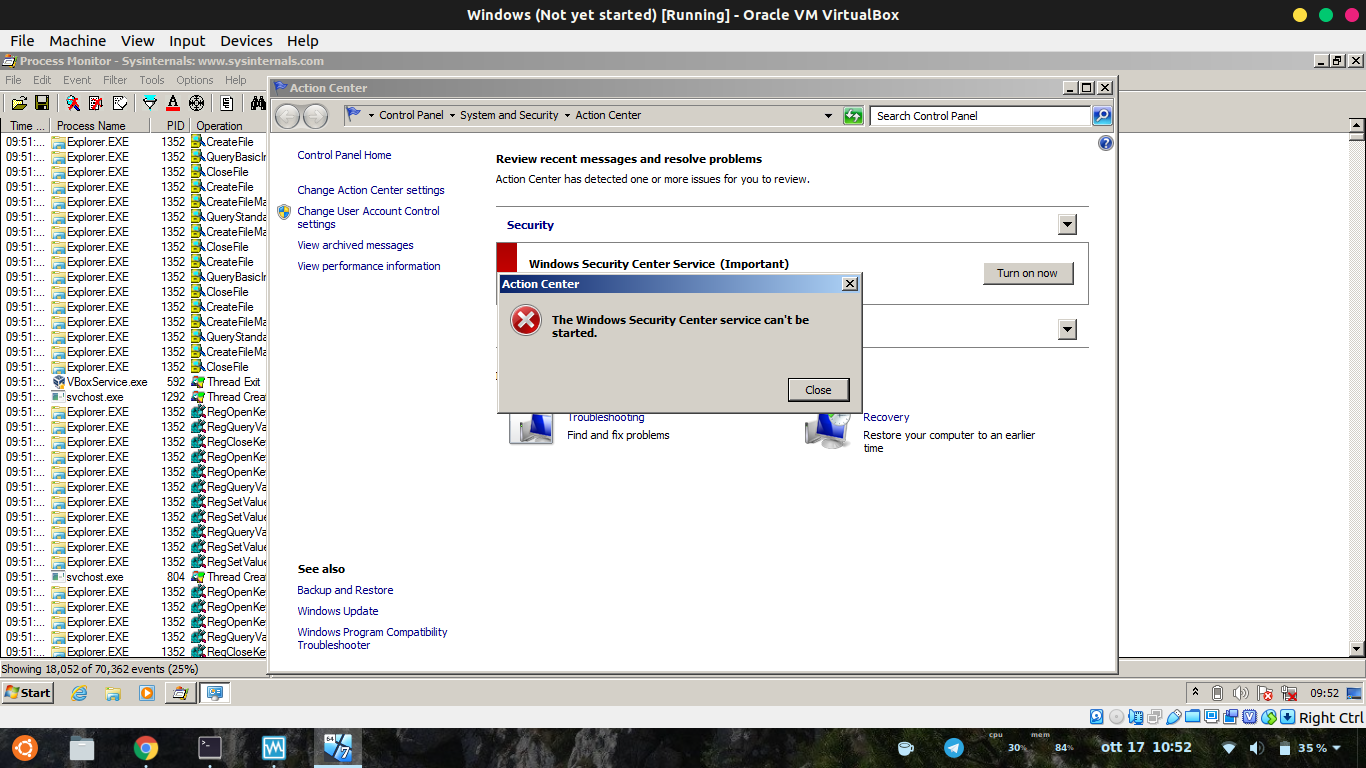
\includegraphics[height=12em]{../img/securityCenter2.png}
	\end{figure}

	After a little bit the \textbf{Windows Security Center} was deactivated.
	\pause

	It could not be restarted.

	\pause

	The malware needs time to perform those actions.

\end{frame}
%-------------------------------------------------------------------------------

\begin{frame}{Fakenet}
	
	With fakenet we registered many POST requests.\\	
	More than 900, to 300 different destinations.
	\pause

	Every request contains:

	\begin{itemize}
		\item Request type
		\item Destination URL
		\item Protocol
		\item User agent
	\end{itemize}
	\pause

	Here's an example:

	\begin{quote}
		\texttt{User-Agent: Mozilla/4.0\\ (compatible; MSIE 28;\dots}
	\end{quote}

	\pause
	There are not imported libraries to send HTTP requests

	\pause 
	\begin{quote}
		$\longrightarrow$ dynamically imported
	\end{quote}
		
\end{frame}
%-------------------------------------------------------------------------------

\begin{frame}{Procmon}
	We used procmon to keep track of every action made by the malware\\
	Dividing them in 3 categories:
	\begin{itemize}
		\item DLL
		\item Registry
		\item Files
	\end{itemize}
\end{frame}
%-------------------------------------------------------------------------------

\begin{frame}{DLL}
	We measured 46 different dll files loaded with the \emph{LoadImage} primitive.

	Among them the most interesting are:

	\begin{itemize}
		\item \textbf{cryptbase - crypt32}: to handle cryptography
		\item \textbf{ws2\_32}: to manage web socket
	\end{itemize}
\end{frame}
%-------------------------------------------------------------------------------

\begin{frame}{Registry}
	We saw many open-read-close actions on many system registers, but only a few write
	\pause

	The only keys modified were:
	\begin{itemize}
		\item Language list, which has no interesting effects
		\item Windows internet zones set to 0 which means \emph{Allow anything} for each network type
	\end{itemize}
\end{frame}
%-------------------------------------------------------------------------------

\begin{frame}{Files}
	We detect the infection of other files watching the ``WriteFile'' operations and the amount of bytes written.

	We obtained the sequence of actions that the malware implement to infect other files

	\pause
	\begin{itemize}
		\item Read the \emph{.exe} victim file.
		\item Write of the content plus the infected part in a \emph{.vir} file with the same name.
		\item Copy of the content of the \emph{.vir} file to the \emph{.exe} one changing the EOF location.
		\item Set of fake information on the executable such as creation and last access time.
		\item Delete the \emph{.vir} file.
	\end{itemize}

\end{frame}
%-------------------------------------------------------------------------------

\begin{frame}{Files}
	The infected files were many, and in different location.

	They were mainly common executables, run frequently by the average user.
	\pause

	The main ones were:

	\begin{itemize}
		\item Windows Media Player
		\item Internet Explorer
		\item Windows Defender
		\item Windows Mail
		\item Windows Photo Viewer
		\item and more\dots
	\end{itemize}

	We inspect the infected files with pestudio and we found a new section called \textbf{.vmp0}

\end{frame}
%-------------------------------------------------------------------------------

\begin{frame}{Regshot}
	With regshot we had a confirmation of all the actions tracked with procmon.

	The fact that caught our attention was the registry change related to the Windows Security Center.

	\texttt{HKLM\textbackslash System\textbackslash CurrentControlSet\textbackslash services\textbackslash wscsvc\textbackslash Start}	$=$ 4

	The value 4 means disabled.

	\pause
	The weird thing is that this value change has not been made by the malware.

	We discovered that the value was changed by \textbf{services.exe}

\end{frame}
%-------------------------------------------------------------------------------

%===============================================================================
\section{Reverse engineering}
\begin{frame}{Reverse engineering}

	The reverse engineering was divided in 2 phases:

	\begin{itemize}
		\item Code rebuilding
		\item Debugging
	\end{itemize}

\end{frame}
%-------------------------------------------------------------------------------

\begin{frame}{Code rebuilding}

	We explored the cfg of the start funcion created by IDA, and we built a pseudo code for the first part, which deals with the decryption of the obfuscated zone.

	% TODO listing

	\pause
	The \emph{.vmp0} section is decrypted through a cycle that perform an arithmetic xor of the code with a certain key. 
	
	The cycle is repetead 7 times, but during the last one the key is incremented by one. 
	
	The key is $0x58$.

\end{frame}
%-------------------------------------------------------------------------------

\begin{frame}{Debugging}

	To debug the code we used Ollydbg alongside procmon, executing instructions one by one, stepping over the function calls and keeping track of the actions performed.

	We had 2 main target:
	\begin{itemize}
		\item Detect the infection function
		\item Detect the deactivation of the security center
	\end{itemize}
\end{frame}
%-------------------------------------------------------------------------------

\begin{frame}{Debugging}
	Eventually we achieved a procedure to debug the infection function:
	\begin{enumerate}
		\item  breakpoint in $0101273A$; then after the \emph{RET} the malware enters the obfuscated section.
		\item breakpoint in $010AAB30$; then there is the creation of the second thread which is the analyzed one.
		\item breakpoint in $010BD0A9$ which is the begin of the target function
	\end{enumerate}

	\pause
	In particular we discovered that the thread calls FUN\_010ACABF, which then calls FUN\_0109F059, which then calls iteratively FUN\_010B0CAD; this last one contains FUN\_010BD0A9 which is the target function that performs the malicious actions.
\end{frame}
%-------------------------------------------------------------------------------

\begin{frame}{Infection}
	The infection function is FUN\_10BD636. 
	
	It has only the target name as parameter. 
	
	\pause
	This procedure is huge, with too much code to reverse; it even contains a recursive call inside.
\end{frame}
%-------------------------------------------------------------------------------

\begin{frame}{Security center dectivation}

	We set the procmon filters to monitor ``services.exe'', and in particular the ``RegSetValue'' operation.

	\pause
	The malicious action is done at $010B10C7$. The third time that this instruction is executed the security center is deactivated

	This action is a call to \textbf{StartServiceA} from \textbf{ADVAPI32.dll}.

	\pause
	Reading the documentation we discovered that this function needs priviledge to close services

	\pause
	\begin{quote}
		$\longrightarrow$ probable priviledge escalation
	\end{quote}

\end{frame}
%-------------------------------------------------------------------------------

\begin{frame}{Conclusions}
	\begin{figure}
		\centering
		\begin{subfigure}{0.475\textwidth}
		  \centering
		  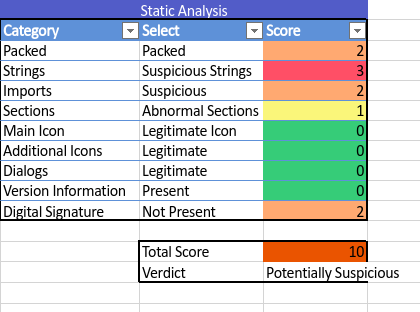
\includegraphics[height=10em]{../img/summary.png}
		\end{subfigure}
		\hfill
		\begin{subfigure}{0.475\textwidth}
		  \centering
		  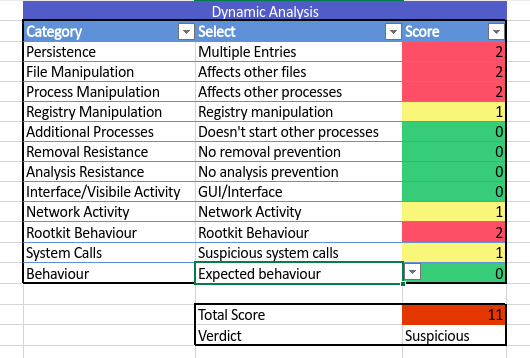
\includegraphics[height=10em]{../img/summary1.png}
		\end{subfigure}
		%\caption{Summary of malware's main features and suspicious behaviours.}
	\end{figure}

	Summing up the result of our analysis we can describe the malware as a polymorphic one, which performs variuos malicious actions such as internet connections, replications on other system programs and deactivates the security center. It disguise itself as a calculator, fooling the average user.

\end{frame}
%-------------------------------------------------------------------------------

\begin{frame}
	
\end{frame}

\end{document}